\documentclass{article}
\usepackage[a4paper, total={6in, 8in}]{geometry}
\usepackage{amsmath} 
\usepackage{graphicx}
\graphicspath{ {./} }

\title{Buying New Car}
\author{Elie Daher}

\begin{document}
\pagenumbering{gobble}
\maketitle
\abstract This document contains the problem of buying a new car from the summary of UTA. This document was made during my internship at LAMSADE in the summer of 2017.\\

A DM wants to buy a new car. The DM is interested only in the following criteria:
\begin{itemize}
\item price (in Euro)
\item comfort ($0$, +, ++, +++) \textit{0 being not comfortable and +++ very comfortable}
\item safety ($1, 2, 3, 4, 5$) \textit{1 being not safety and 5 safe}
\end{itemize}
The evaluation of the previous criteria is presented in the following table: 
\begin{center}
 \begin{tabular}{|c | c c c c|} 
 \hline
 Cars & Price & Comfort & Safety & Ranking of the DM \\ [0.5ex] 
 \hline
 Nissan Sentra (ns) & 17\,000 & +++ & 4 & 1 \\ 
 \hline
 Citroen C4 (c4) & 15\,000& ++ & 2 & 2\\ 
 \hline
 Peugeot 208 GT (p208) & 25\,000 & + & 3 & 3\\
 \hline
 Peugeot 308 berline (p308)& 18\,500 & 0 & 3 & 4\\
 \hline
\end{tabular}
\end{center}
\newpage
First of all, we should specify the scale \footnote{the interval $[g_{i*}, g_{i}^{*}]$ is cut into equal intervals} for each criteria.
\begin{itemize}
\item Price $\quad \Rightarrow \quad [g_{1*}, g_{1}^{*}] = [25\,000, 20\,000, 15\,000]$
\item Comfort $\quad \Rightarrow \quad [g_{2*}, g_{2}^{*}] = [0, +, ++, +++]$
\item Safety $\quad \Rightarrow \quad [g_{3*}, g_{3}^{*}] = [1, 3, 5]$
\end{itemize}
According to this formula: $v(g(a)) = \sum_{i=1}^{n} v_i (g_i (a))$ , the value of each alternative may be written: 
\begin{itemize}
\item $v(g(ns)) =  0.4v_1(15\,000) +  0.6v_1(20\,000) + v_2(+++) + 0.5v_3(3) + 0.5v_3(5)  $
\item $v(g(c4)) = v_1(15\,000) + v_2(++) + 0.5 v_3(1) + 0.5v_3(3) = v_1(15\,000) + v_2(++) + 0.5v_3(3)$
\item $v(g(p208)) = v_1(25\,000) + v_2(+) + v_3(3) = v_2(+) + v_3(3) $
\item $v(g(p308)) = 0.3v_1(15\,000) +  0.7v_1(20\,000) + v_2(0) + v_3(3) = 0.3v_1(15\,000) +  0.7v_1(20\,000) + v_3(3)$
\end{itemize}
We have that $v_1(25\,000) = v_2(0) = v_3(1) = 0$. \\
Since the marginal value $u_i(g_i)$ can be expressed in terms of variables $w_{ij}$: $u_i(g_i^{j}) = \sum _{t=1}^{j-1} w_{it}$ , the value of each alternatie can be written: 
\begin{itemize}
\item $v(g(ns)) = w_{11} + 0.4w_{12} + w_{21} + w_{22} + w_{23} + w_{31} + 0.5w_{32}$
\item $v(g(c4)) = w_{11} + w_{12} + w_{21} + w_{22} + 0.5w_{31}$
\item $v(g(p208)) = w_{21} + w_{31} $
\item $v(g(p308)) = w_{11} + 0.3w_{12} + w_{31}$
\end{itemize}
For each pair of consecutive alternatives, we express the difference between them: 
\begin{itemize}
\item $\Delta (ns,c4) =  -0.6w_{12} + w_{23} + 0.5w_{31} +  0.5w_{32}  -\sigma _{ns}^{+} +\sigma _{ns}^{-} +\sigma _{c4}^{+} - \sigma _{c4}^{-} $
\item $\Delta (c4, p208) = w_{11} + w_{12} + w_{22} - 0.5w_{31} -\sigma _{c4}^{+} +\sigma _{c4}^{-} +\sigma _{p208}^{+} - \sigma _{p208}^{-} $
\item $\Delta (p208, p308) =w_{21} - w_{11} - 0.3w_{12} -\sigma _{p208}^{+} +\sigma _{p208}^{-} +\sigma _{p308}^{+} - \sigma _{p308}^{-} $
\end{itemize}
Having $\delta = 0.05$, we can solve the following LP:\\

Objective:  
\begin{equation}
	Minimize \quad \sum_{a \in A} \sigma _{a}^{+} + \sigma _{a}^{-}
\end{equation}

Subject to: \\
\begin{equation}
	\begin{cases}
		 -0.6w_{12} + w_{23} + 0.5w_{31} + 0.5w_{32}  -\sigma _{ns}^{+} +\sigma _{ns}^{-} +\sigma _{c4}^{+} - \sigma _{c4}^{-}   \geq 0.05\\
		w_{21} - w_{11} - 0.3w_{12} -\sigma _{p208}^{+} +\sigma _{p208}^{-} +\sigma _{p308}^{+} - \sigma _{p308}^{-}  \geq 0.05 \\
		- 0.1w_{12} - w_{21} - w_{22} - w_{23} - 0.5w_{32} -\sigma _{p308}^{+} +\sigma _{p308}^{-} +\sigma _{ns}^{+} - \sigma _{ns}^{-}  \geq 0.05 \\
		w_{11} + w_{12} + w_{21} + w_{22} + w_{23} + w_{31} + w_{32} = 1
	\end{cases}
\end{equation}
So by using the com.google.ortools library, we can solve the Linear Program above with $\sigma = 0.05$. This Linear Program solution is coded in Java class BuyingNewCar.\\
By executing the class BuyingNewCar, you will have the following result: \\
\begin{center}
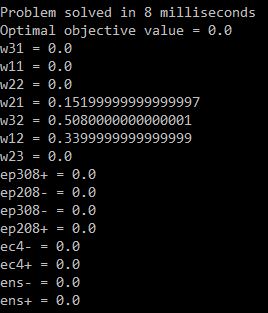
\includegraphics[height=6.5cm]{result.png}
\end{center}
An optimal solution is $w_{12} = 0.34$, $w_{21} = 0.152$, $w_{31} = 0.51$ with $\sum_{a \in A} \sigma _{a}^{+} + \sigma _{a}^{-} = 0$. The utilities found for each alternative are as follows: \\ 
\begin{itemize}
\item $v(g(ns)) = 0.798$
\item $v(g(c4)) = 0.747$
\item $v(g(p208)) = 0.662 $
\item $v(g(p308)) = 0.62 $
\end{itemize}
Those utilities are consistent with the DM's preference ranking. \\

\end{document}